\chapter{Resultados}
\label{ch:resultados}
\section{Desempe\~no}
En esta secci\'on se describen los resultados obtenidos durante las experiencias de medici\'on de desempe\~no de la nueva versi\'on del programa en t\'erminos de tiempo y memoria principal usada. 
\bigskip

Las pruebas se realizaron usando el mismo conjunto de datos utilizado para medir el desempe\~no del programa original 
(Cap\'itulo \ref{ch:prev_work}), adem\'as se emplearon como herramientas de medici\'on igualmente el perfilador de memoria \texttt{mem\_profiler} y la librer\'ia \textsc{Resource}\footnote{M\'etodo \texttt{get\_rusage}}.

\subsection{Filtros b\'asico y de m\'axima correntrop\'ia}

Las Tablas \ref{tab:t7} y \ref{tab:t9} muestran los resultados de tiempo medido en segundos de cada una de las partes del proceso de la rutina principal, para los tres datasets usando los filtros b\'asico y de m\'axima correntrop\'ia, respectivamente. Posteriormente, las Tablas \ref{tab:t8} y \ref{tab:t10} resumen la totalidad de tiempo usado durante la ejecuci\'on (para ambos filtros). A todos estos resultados se les ha agregado la medici\'on de tiempo promedio utilizado por imagen (ya que las secuencias poseen largos diferentes). 

\begin{table}[h!]
\centering
\caption{Tiempo de ejecuci\'on en segundos de cada proceso involucrado, usando el filtro de Kalman b\'asico refactorizado: c\'alculo de flujo estimaci\'on de filtros, agrupaci\'on de pixeles y obtenci\'on de candidatos (operaci\'on que involucra guardado de los mismos). La \'ultima fila describe el tiempo promedio que toma por observaci\'on (en segundos igualmente) para cada uno de los procesos. }
\begin{tabular}{|l|l|l|l|l|}
\hline
\textbf{ID} & \textbf{C\'alc. Flujos [s]} & \textbf{Aplic. KF [s]} &  \textbf{Agrup. Pixeles [s]}  & \textbf{Obt. Candidatos [s]}\\ \hline \hline
SN14        & 285.81            & 22.45        &  65.18 & 0.00 \\ \hline
SN18            & 253.19             & 20.08         &  65.67  & 0.00\\ \hline
SN80            & 228.60             & 26.06         &   67.77 & 0.00 \\ \hline \hline
%Media & 303.08 &  26.23 & 37.83 & 0.01\\\hline 
$\bar{t}/Obs$ & 11.57 &  1.06 & 3.04 & 0.00\\\hline 
\end{tabular}
\label{tab:t7}
\end{table}


\begin{table}[h!]
\centering
\caption{Tiempo de ejecuci\'on de los procesos de b\'usqueda de supernova de HiTS, revisi\'on de los candidatos encontrados y tiempo total comprendido por ambos procesos usando filtro de Kalman B\'asico refactorizado. La \'ultima fila corresponde a tiempo total promedio por observaci\'on.}
\begin{tabular}{|l|l|}
\hline
\textbf{ID} & \textbf{Tiempo total} \\ \hline
\hline
SN14  & 373.44 \\\hline
SN18  & 338.94\\\hline
SN80  & 322.43 \\\hline\hline
%Media & 367.15 & 374.83 & 741.98  \\\hline
 $\bar{t}/Obs. $& 15.67 \\\hline 
\end{tabular}
\label{tab:t8}

\end{table}

Las figuras \ref{fig:mem_new_kbf} y \ref{fig:mem_new_mcc} muestran el comportamiento del consumo de memoria para la nueva versi\'on del filtro b\'asico y de m\'axima correntrop\'ia, respectivamente, ejecutando la pipeline refactorizada sobre los tres conjuntos de datos (SN14, SN18 y SN80). 

\begin{figure}[h!]
\centering
\subfloat[Memoria ocupada en SN14]{\label{fig:new_kbf_14}{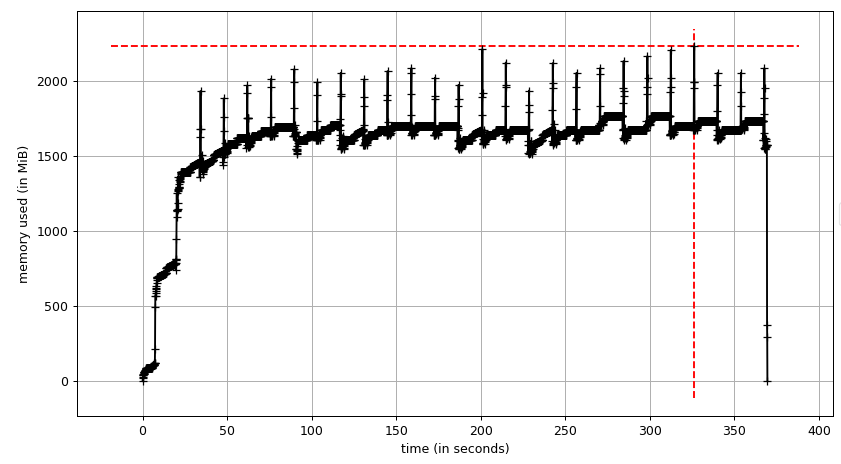
\includegraphics[width=0.5\textwidth]{images/results/sn14_new_bk}}}\hfill
\subfloat[Memoria ocupada en SN18]{\label{fig:new_kbf_18}{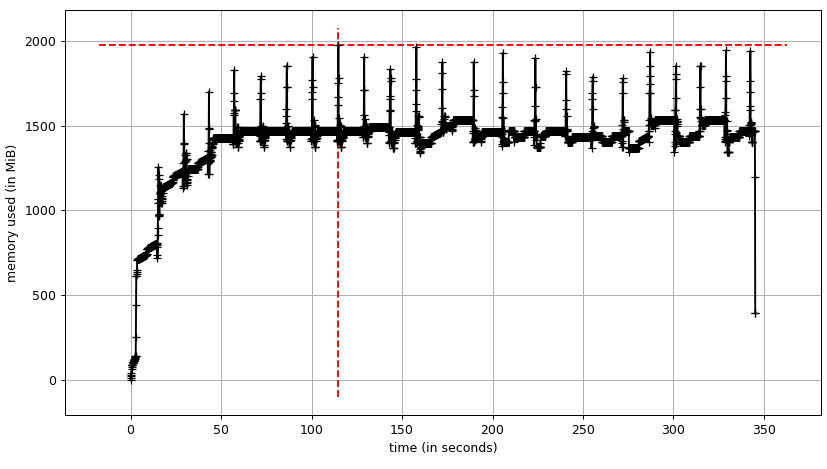
\includegraphics[width=0.5\textwidth]{images/results/sn18_new_bk}}}\vfill
\subfloat[Memoria ocupada en SN80]{\label{fig:new_kbf_80}{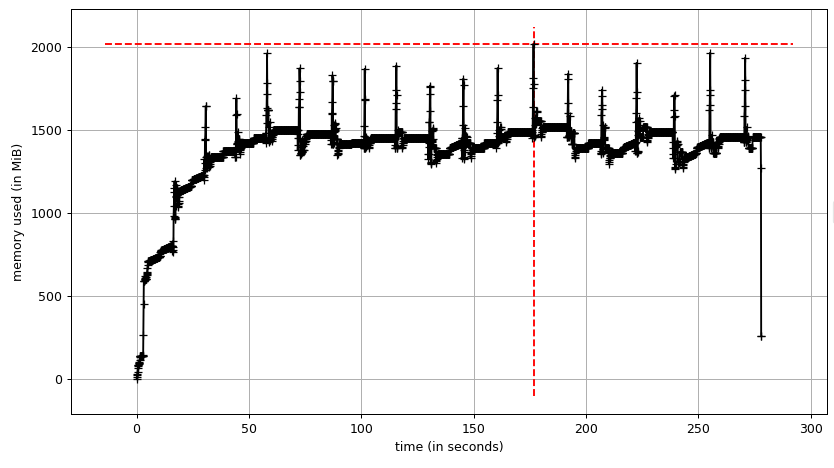
\includegraphics[width=0.5\textwidth]{images/results/sn80_new_bk}}}
\caption{Comportamiento de la memoria (en mebibytes) durante la ejecuci\'on para los tres conjuntos de datos usando el filtro de Kalman B\'asico.}
\label{fig:mem_new_kbf}
\end{figure}

\begin{table}[h!]
\centering
\caption{Memoria principal (en unidades de MB) usada durante la ejecuci\'on del programa refctorizado usando filtro de Kalman B\'asico.}
\begin{tabular}{|l|l|}
\hline
\textbf{ID} & Memoria [MB]\\\hline\hline
SN14 & 2098.00\\\hline
SN18 & 2066.72\\\hline
SN80 & 2119.24\\\hline
\end{tabular}
\label{tab:mem3}
\end{table}

\begin{table}[h!]
\centering
\caption{Tiempo de ejecuci\'on en segundos de cada proceso involucrado, usando el filtro de Kalman de m\'axima correntrop\'ia refactorizado: c\'alculo de flujo estimaci\'on de filtros, agrupaci\'on de pixeles y obtenci\'on de candidatos (operaci\'on que involucra guardado de los mismos). La \'ultima fila describe el tiempo promedio que toma por observaci\'on (en segundos igualmente) para cada uno de los procesos. }
\begin{tabular}{|l|l|l|l|l|}
\hline
\textbf{ID} & \textbf{C\'alc. Flujos [s]} & \textbf{Aplic. KF [s]} &  \textbf{Agrup. Pixeles [s]}  & \textbf{Actual. Candidatos [s]}\\ \hline \hline
SN14        & 284.99            & 529.68        &  54.86 & 0.00 \\ \hline
SN18            & 256.58             & 507.46         &  66.73  & 0.00\\ \hline
SN80            & 209.02             & 411.94         &   45.94 & 0.00 \\ \hline \hline
%Media & 303.08 &  26.23 & 37.83 & 0.01\\\hline 
$\bar{t}/Obs$ & 11.00 &  0.97 & 2.24 & 0.00\\\hline 
\end{tabular}
\label{tab:t9}
\end{table}

\begin{table}[h!]
\centering
\caption{Tiempo de ejecuci\'on de los procesos de b\'usqueda de supernova de HiTS, revisi\'on de los candidatos encontrados y tiempo total comprendido por ambos procesos usando filtro de Kalman de m\'axima correntrop\'ia refactorizado. La \'ultima fila corresponde a tiempo total promedio por observaci\'on.}
\begin{tabular}{|l|l|}
\hline
\textbf{ID} & \textbf{Tiempo total} \\ \hline
\hline
SN14  & 869.53 \\\hline
SN18  & 830.77\\\hline
SN80  & 666.90 \\\hline\hline
%Media & 367.15 & 374.83 & 741.98  \\\hline
 $\bar{t}/Obs. $& 35.54 \\\hline 
\end{tabular}

\label{tab:t10}
\end{table}

\begin{figure}[h!]
\centering
\subfloat[Memoria ocupada en SN14]{\label{fig:new_mcc_14}{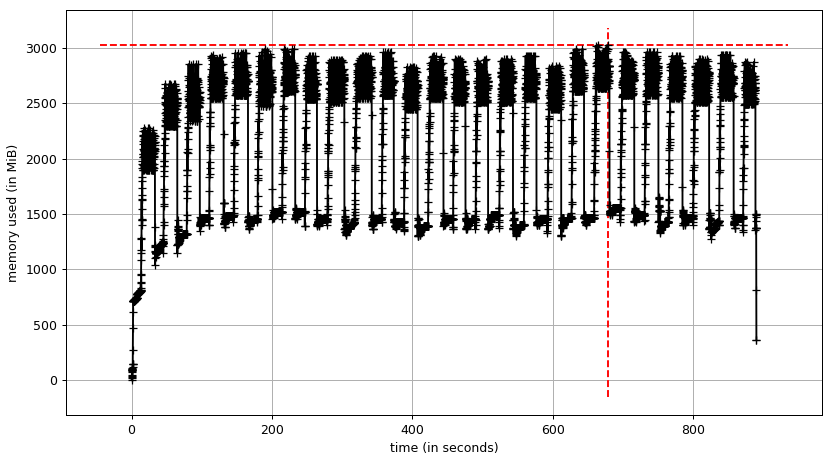
\includegraphics[width=0.5\textwidth]{images/results/sn14_new_mcc}}}\hfill
\subfloat[Memoria ocupada en SN18]{\label{fig:new_mcc_18}{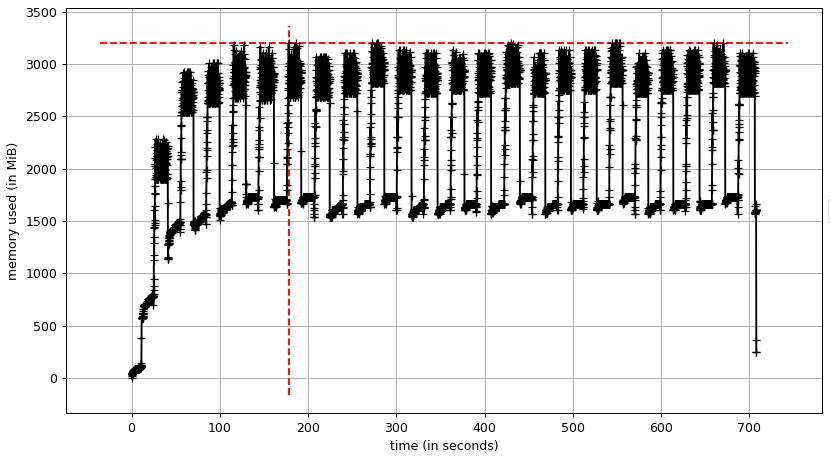
\includegraphics[width=0.5\textwidth]{images/results/sn18_new_mcc}}}\vfill
\subfloat[Memoria ocupada en SN80]{\label{fig:new_mcc_80}{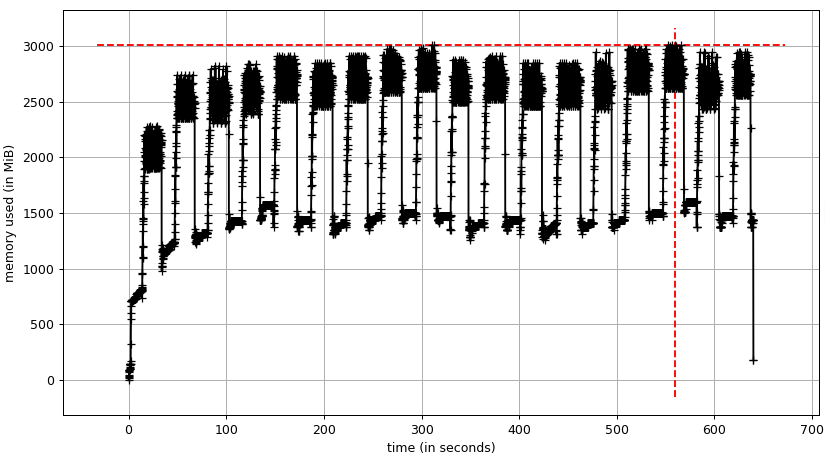
\includegraphics[width=0.5\textwidth]{images/results/sn80_new_mcc}}}
\caption{Comportamiento de la memoria (en mebibytes) durante la ejecuci\'on para los tres conjuntos de datos. En los tres lanzamientos se us\'o el filtro de Kalman de m\'axima correntrop\'ia.}
\label{fig:mem_new_mcc}
\end{figure}

\begin{table}[h!]
\centering
\caption{Memoria principal (en unidades de MB) usada durante la ejecuci\'on del programa refactorizado usando filtro de Kalman de m\'axima correntrop\'ia.}
\begin{tabular}{|l|l|}
\hline
\textbf{ID} & Memoria [MB]\\\hline\hline
SN14 & 3164.83\\\hline
SN18 & 3186.06\\\hline
SN80 & 3154.98\\\hline
\end{tabular}
\label{tab:mem4}
\end{table}

\subsection{Filtro unscented}
Actualmente se est\'an realizando pruebas de correctitud del filtro (\texttt{unittests}). Una vez que las pruebas sean pasadas se ejecutar\'an las pruebas de desempe\~no.
\section{Pruebas en Leftraru}
A continuaci\'on se detallan los resultados obtenidos para esta nueva pipeline sobre los datos en las 93 supernovas conocidas. Para todos los filtros listados se emple\'o un threshold de flujo de 200 y de velocidad de flujo de 50.
\subsection{Filtros b\'asico y de m\'axima correntrop\'ia}
La Tabla \ref{tab:tpfn_new} muestra los resultados obtenidos con la nueva versi\'on de la pipeline, empleando los filtros refactorizados de la familia strategy.
\begin{table}[h!]
\centering
\caption{N\'umero de falsos negativos (FN) y verdaderos positivos (TP) encontrados usando cada uno de los filtros. No se observan diferencias entre los resultados de cada filtro refactorizado. La tercera columna de valores muestra la cantidad de conjuntos de datos que no puedieron ser procesados.}
\begin{tabular}{|l|l|l|l|}
\hline
\textbf{Filtro} & \textbf{TP} & \textbf{FN} & \textbf{NaN}\\ \hline
Básico          & 37          & 56          &  3 \\ \hline
MCC             & 37          & 56          & 3 \\ \hline
\end{tabular}
\label{tab:tpfn_new}
\end{table}
\bigskip

Los resultados muestran que para el programa refactorizado tanto el filtro b\'asico como el de correntrop\'ia m\'axima detectan la misma cantidad de supernovas de HiTS. De acuerdo a la informaci\'on dispuesta en la secci\'on \ref{ap:pip_ref} ap\'endice, donde se muestra la tabla \ref{ap:tab2}, se desprende que tampoco hay diferencias de los tiempos o \'epocas de detecci\'on.
\bigskip

Al comparar las tablas \ref{ap:tab1}, correspondiente a los tiempos de detecci\'on en MJD de las implementaciones originales de los filtros y \ref{ap:tab2} a los tiempos de las versiones refactorizadas, se deduce que las detecciones con el \'ultimo grupo de filtros ocurren, cuando es el caso, en la misma \'epoca o antes (horas o d\'ias). Por ejemplo, en las im\'agenes \ref{fig:orig_det_snL} y  \ref{fig:orig_det_snaa} las detecciones se realizan en 57072.145 y 57075.12 con el nuevo conjunto de filtros.
En otras ocasiones, alguno de los grupos no detecta la supernova y en el peor de los casos ninguno de los dos reconoce la supernova.
\bigskip
  

\subsection{Filtro unscented}
Una vez que se pasen las pruebas (\texttt{unittests}) de correctitud, se proceder\'a a ejecutar las pruebas del filtro Unscented en Leftraru.